 % !TeX program = pdflatex
\documentclass[11pt]{article}

% ---- Aesthetics & layout ----
\usepackage[margin=1in]{geometry}
\usepackage{lmodern}
\usepackage{microtype}
\usepackage{setspace}
\onehalfspacing

% ---- Math & theorems ----
\usepackage{amsmath, amssymb, mathtools, bm}
\usepackage{amsthm}
\numberwithin{equation}{section}

% ---- Figures, tables, algorithms ----
\usepackage{xcolor}
\usepackage{graphicx}
\usepackage{tikz}
\usetikzlibrary{arrows.meta,calc,fit,positioning}
\usepackage{subcaption}
\usepackage{array}
\usepackage{tabularx}
\usepackage{booktabs}
\usepackage{float}
\usepackage{algorithm}
\usepackage{algorithmic}

% ---- Diagram palette ----
\definecolor{qnavy}{HTML}{17365D}
\definecolor{qnavysoft}{HTML}{355374}
\definecolor{qteal}{HTML}{1B7F83}
\definecolor{qtealdark}{HTML}{0B5D63}
\definecolor{qgold}{HTML}{B9831F}
\definecolor{qgolddark}{HTML}{8A610D}
\definecolor{qink}{HTML}{1F252B}
\definecolor{qmuted}{HTML}{667085}
\definecolor{qpanel}{HTML}{F7F9FC}
\definecolor{qtealfill}{HTML}{EFF7F6}
\definecolor{qgoldfill}{HTML}{FFF8EA}
\definecolor{qline}{HTML}{CFD8E3}

% ---- Citations & hyperlinks ----
\usepackage[round,authoryear]{natbib}
\usepackage{hyperref}
\hypersetup{colorlinks=true,linkcolor=black,citecolor=black,urlcolor=black}

% ---- Shortcuts (unified notation) ----
\newcommand{\R}{\mathbb{R}}
\newcommand{\E}{\mathbb{E}}
\newcommand{\Normal}{\mathcal{N}}
\newcommand{\TN}{\mathcal{N}^+}
\newcommand{\ind}{\mathbf{1}}
\newcommand{\diag}{\mathrm{diag}}
\newcommand{\vect}[1]{\bm{#1}}
\newcommand{\mat}[1]{\bm{#1}}
\DeclareMathOperator{\argmin}{arg\,min}
\DeclareMathOperator{\Var}{Var}
\DeclareMathOperator{\IG}{IG}
\DeclareMathOperator{\GIG}{GIG}

% Distributions as macros for consistency
\newcommand{\Exp}{\mathrm{Exp}}
\newcommand{\Unif}{\mathrm{Unif}}
\newcommand{\AL}{\mathrm{AL}}
\newcommand{\exAL}{\mathrm{exAL}}
\newcommand{\aCRPS}{\mathrm{aCRPS}}
\newcommand{\RHS}{\ensuremath{\mathrm{RHS}}}
\newcommand{\pkg}[1]{\textsf{#1}}
\newcolumntype{Y}{>{\raggedright\arraybackslash}X}
\newcommand{\TableStyle}{%
  \footnotesize
  \setlength{\tabcolsep}{4.5pt}%
  \renewcommand{\arraystretch}{1.12}%
}

% GloFAS application output aliases.
% Article-facing current-output aliases for the GloFAS application section.
\newcommand{\GlofasApplicationCurrentScoreTable}{tables/glofas_application_current_score_summary.tex}
\newcommand{\GlofasApplicationCurrentCorrectedPathsFigure}{figures/glofas_application/glofas_qdesn_discrepancy_corrected_quantile_paths__glofas_stage_n_winner_scorebalanced_20260703.pdf}
\newcommand{\GlofasApplicationCurrentForecastWindowFigure}{figures/glofas_application/diagnostics/glofas_stage_n_winner_full7_scorebalanced_qdesn_synthesized_bands__glofas_stage_n_winner_scorebalanced_20260703.pdf}
\newcommand{\GlofasApplicationCurrentQdesnCheckLoss}{0.3339}
\newcommand{\GlofasApplicationCurrentRawCheckLoss}{0.7639}
\newcommand{\GlofasApplicationCurrentCheckLossReduction}{56.3\%}
\newcommand{\GlofasApplicationCurrentQdesnIntervalScore}{4.1402}
\newcommand{\GlofasApplicationCurrentRawIntervalScore}{13.0538}
\newcommand{\GlofasApplicationCurrentIntervalScoreReduction}{68.3\%}
\newcommand{\GlofasApplicationCurrentQdesnCrps}{0.6859}
\newcommand{\GlofasApplicationCurrentRawCrps}{1.4424}
\newcommand{\GlofasApplicationCurrentCrpsReduction}{52.4\%}
\newcommand{\GlofasApplicationCurrentQdesnMeanCoverage}{0.833}
\newcommand{\GlofasApplicationCurrentRawMeanCoverage}{0.000}
\newcommand{\GlofasApplicationCurrentScoredHorizons}{28}
\newcommand{\GlofasApplicationCurrentOriginDate}{2022-12-25}
\newcommand{\GlofasApplicationCurrentVbIterations}{median 150; max 150}
\newcommand{\GlofasApplicationCurrentReferenceReservoirDepth}{4}
\newcommand{\GlofasApplicationCurrentReferenceReservoirSize}{100,100,100,100}
\newcommand{\GlofasApplicationCurrentReferenceReducerSize}{100,100,100}
\newcommand{\GlofasApplicationCurrentReferenceReservoirMemory}{300}
\newcommand{\GlofasApplicationCurrentReferenceReservoirWashout}{500}
\newcommand{\GlofasApplicationCurrentReferenceReservoirAlpha}{0.0225,0.0225,0.0225,0.0225}
\newcommand{\GlofasApplicationCurrentReferenceReservoirRho}{0.95,0.95,0.95,0.95}
\newcommand{\GlofasApplicationCurrentReferenceReservoirPiW}{0.03,0.03,0.03,0.03}
\newcommand{\GlofasApplicationCurrentReferenceReservoirPiIn}{1,1,1,1}
\newcommand{\GlofasApplicationCurrentReferenceReservoirWinScaleGlobal}{0.16}
\newcommand{\GlofasApplicationCurrentReferenceReservoirWinScaleBias}{0.16}
\newcommand{\GlofasApplicationCurrentReferenceReservoirSeed}{20260512}
\newcommand{\GlofasApplicationCurrentDiscrepancyReservoirDepth}{4}
\newcommand{\GlofasApplicationCurrentDiscrepancyReservoirSize}{100,100,100,100}
\newcommand{\GlofasApplicationCurrentDiscrepancyReducerSize}{100,100,100}
\newcommand{\GlofasApplicationCurrentDiscrepancyReservoirMemory}{300}
\newcommand{\GlofasApplicationCurrentDiscrepancyReservoirWashout}{500}
\newcommand{\GlofasApplicationCurrentDiscrepancyReservoirAlpha}{0.0075,0.0075,0.0075,0.0075}
\newcommand{\GlofasApplicationCurrentDiscrepancyReservoirRho}{0.95,0.95,0.95,0.95}
\newcommand{\GlofasApplicationCurrentDiscrepancyReservoirPiW}{0.03,0.03,0.03,0.03}
\newcommand{\GlofasApplicationCurrentDiscrepancyReservoirPiIn}{1,1,1,1}
\newcommand{\GlofasApplicationCurrentDiscrepancyReservoirWinScaleGlobal}{0.28}
\newcommand{\GlofasApplicationCurrentDiscrepancyReservoirWinScaleBias}{0.28}
\newcommand{\GlofasApplicationCurrentDiscrepancyReservoirSeed}{20261521}
\newcommand{\GlofasApplicationCurrentSharedRhsTau}{0.001}
\newcommand{\GlofasApplicationCurrentDiscrepancyRhsTau}{0.03}
\newcommand{\GlofasApplicationCurrentSpreadCalibrationFactor}{1.4}
\newcommand{\GlofasApplicationCurrentSpreadCalibrationAdditiveWidth}{0.5}
\newcommand{\GlofasApplicationCurrentSpreadCalibrationCenterQuantile}{0.50}

% PriceFM application output aliases.
% Reported current-output aliases for the full PriceFM benchmark section.
\newcommand{\PricefmFullRegionFolds}{114}
\newcommand{\PricefmFullRegions}{38}
\newcommand{\PricefmFullFolds}{3}
\newcommand{\PricefmFullQdesnWins}{66}
\newcommand{\PricefmFullQdesnClose}{12}
\newcommand{\PricefmFullPricefmWins}{36}
\newcommand{\PricefmFullQdesnWinRate}{57.9\%}
\newcommand{\PricefmFullMeanQdesnAql}{6.826}
\newcommand{\PricefmFullMeanPricefmAql}{7.039}
\newcommand{\PricefmFullMeanDeltaAql}{-0.213}
\newcommand{\PricefmFullMedianDeltaAql}{-0.083}
\newcommand{\PricefmFullGraphRows}{56}
\newcommand{\PricefmFullTargetOnlyRows}{58}
\newcommand{\PricefmFullHorizonRows}{72}
\newcommand{\PricefmFullPaperQuantiles}{0.10, 0.25, 0.45, 0.50, 0.55, 0.75, 0.90}
\newcommand{\PricefmFullMainSummaryTable}{tables/pricefm_full_main_summary.tex}

% PriceFM matched-comparison aliases.
\newcommand{\PricefmPaperAlignedMainComparisonTable}{tables/pricefm_paper_aligned_main_comparison.tex}
\newcommand{\PricefmAlignedQdesnAqcr}{2.58\%}
\newcommand{\PricefmAlignedPricefmAqcr}{0.00\%}
\newcommand{\PricefmAlignedQdesnMae}{16.722}
\newcommand{\PricefmAlignedPricefmMae}{17.274}
\newcommand{\PricefmAlignedQdesnRmse}{25.449}
\newcommand{\PricefmAlignedPricefmRmse}{26.336}
\newcommand{\PricefmAlignedAqlReduction}{3.1\%}
\newcommand{\PricefmAlignedMaeReduction}{3.2\%}
\newcommand{\PricefmAlignedRmseReduction}{3.4\%}


% Identity, zeros, and ones with consistent bold style
\newcommand{\Id}[1]{\mat I_{#1}}
\newcommand{\zeros}[1]{\vect 0_{#1}}
\newcommand{\ones}[1]{\vect 1_{#1}}

% ---- Theorem-style environments ----
\theoremstyle{plain}
\newtheorem{theorem}{Theorem}[section]
\newtheorem{proposition}[theorem]{Proposition}
\newtheorem{lemma}[theorem]{Lemma}
\theoremstyle{definition}
\newtheorem{definition}[theorem]{Definition}
\newtheorem{assumption}[theorem]{Assumption}
\theoremstyle{remark}
\newtheorem{remark}[theorem]{Remark}

% ---- Title & metadata ----
\title{\vspace{-0.6cm}Bayesian Quantile Deep Echo State Networks\\for Nonlinear Time Series}
\author{Antonio De Leon$^{1}$ \and Raquel Prado$^{1}$ \and Bruno Sans\'o$^{1}$}
\date{\small $^{1}$Department of Statistics, University of California, Santa Cruz \\
\vspace{0.25em}August 28, 2026}

\begin{document}
\maketitle
\vspace{-1.25em}

\begin{abstract}
\noindent
Conditional quantiles are central to asymmetric decision losses, tail-risk
assessment, and interval forecasts, but Bayesian quantile regression for
nonlinear time series can be difficult when the temporal feature vector is
high-dimensional. We develop the quantile deep echo state network (Q--DESN), a
Bayesian quantile regression model conditional on fixed features generated by a
deep echo state network. Conditional on a specified reservoir construction and
feature map, posterior uncertainty is assigned to the regression coefficients,
likelihood, and shrinkage parameters.
Single-level fits use asymmetric Laplace or quantile-fixed generalized
asymmetric Laplace working likelihoods with ridge or regularized-horseshoe
priors. Posterior computation uses Markov chain Monte Carlo when computationally
practical and a model-specific variational Bayes approximation for analyses
requiring repeated fitting. For quantile grids, we compare
independent level-wise regressions followed by monotone rearrangement with a
joint quantile-vector regression that shrinks adjacent quantile-specific
coefficient differences. Synthetic studies, a single-origin retrospective
Global Flood Awareness System (GloFAS) streamflow case, and a retrospective
PriceFM comparison identify
settings where this fixed-feature Bayesian regression improves finite-grid
quantile scores.
\end{abstract}

\bigskip

% ============================================================
\section{Introduction}
\label{sec:intro}

Conditional quantiles are natural summaries for asymmetric decision losses,
tail-risk assessment, and interval forecasts. If \(\mathcal F_t\) is the
information available at forecast origin \(t\), the level-\(p\) quantile of a
future response is
\[
Q_{t,h}(p)=\inf\{u:\Pr(Y_{t+h}\le u\mid\mathcal F_t)\ge p\},
\qquad 0<p<1.
\]
Quantile regression estimates this quantity directly
\citep{KoenkerBassett1978,Koenker2005}. Dynamic applications are more
difficult when nonlinear temporal structure must be represented by a large
number of correlated predictors and inference must be repeated over forecast
origins or probability levels.

Echo state networks (ESNs) represent temporal dependence through recurrent
nonlinear states whose reservoir weights are drawn once rather than estimated
with the regression coefficients
\citep{Jaeger2001EchoState,LukoseviciusJaeger2009ReservoirComputing}. Deep ESNs
stack these reservoirs to obtain features at several time scales
\citep{GallicchioMicheliPedrelli2018DeepESNDesign}. We use the resulting states
as a fixed nonlinear design and place Bayesian quantile regression on the final
linear predictor. This separation retains the computational economy of
reservoir methods while providing regularized posterior inference for the
conditional quantile.

The proposed quantile deep echo state network (Q--DESN) uses either the
asymmetric Laplace (AL) likelihood or the quantile-fixed generalized
asymmetric Laplace likelihood of \citet{yan2025new}, abbreviated exAL. Both are
working likelihoods: they define posterior inference for quantile-regression
parameters without asserting the corresponding error law
\citep{sriram2013theoretical,YangWangHe2016ALInference,JiLeeRabeHesketh2025ValidSE}.
The exAL family adds a shape parameter while preserving the chosen conditional
quantile as its location. Ridge regularization supplies a dense baseline, and
the regularized horseshoe (RHS) supplies adaptive global--local shrinkage with
a finite slab \citep{CarvalhoPolsonScott2010HS,PiironenVehtari2017RHS}.

Several ESN methods already address probabilistic or quantile forecasting
\citep{McDermottWikle2018DeepESNUQ,LvZhaoLiuWang2016QRESNE,
BonasWikleCastruccio2024CalibratedDeepESN}. Q--DESN differs by treating a
specified DESN realization as a fixed feature map and assigning a posterior to
the quantile-specific regression, likelihood, and shrinkage parameters. Its
linear dynamic comparators are the DQLM and exDQLM
\citep{GoncalvesMigonBastos2020DQLM,barata2021_flex_quantile}, implemented in
version 1.1.1 of the CRAN package \pkg{exdqlm} \citep{exdqlmRPackage}.

For a grid of probability levels, we distinguish two inferential strategies.
Independent regressions may be rearranged after fitting to obtain an ordered
reported grid \citep{BarlowBrunk1972IsotonicDual,chernozhukov2010}. A joint
quantile-vector regression instead shares information during estimation by
placing RHS priors on adjacent quantile-specific coefficient differences,
adapting the Quantile-Varying Parameter construction of
\citet{KohnsSzendrei2025QVP}. This prior can reduce crossings but does not
enforce noncrossing; an ordered parameterization or explicit rearrangement is
still required for exact monotonicity
\citep{WuLiu2009StepwiseNCQR,BondellReichWang2010NoncrossingQR,
YangTokdar2017JointQuantilePlanes}.

The article contributes the fixed-feature Bayesian Q--DESN formulation, its
independent and joint quantile-grid variants, and posterior computation by
Markov chain Monte Carlo (MCMC) and a model-specific variational Bayes
approximation. A single-quantile simulation compares Q--DESN with DQLM and
exDQLM; a second simulation isolates joint versus independent estimation of a
seven-level quantile grid. Retrospective GloFAS streamflow and PriceFM
electricity-price examples assess independent Q--DESN regressions under their
stated information sets. The supplement contains the complete posterior
derivations, initialization and forecast details, diagnostics, and full
numerical results.

% ============================================================
\section{Fixed-Feature Bayesian Quantile Models}
\label{sec:model}
\label{sec:notation}

\subsection{Deep echo state network features}
\label{subsec:desn}

Let \(\vect u_t=(y_{t-1},\ldots,y_{t-m},\vect z_t^\top)^\top\) contain response
lags and exogenous variables. For layer \(d\), \(\bar{\mat W}_d\) is a fixed
sparse recurrent matrix scaled to target spectral radius \(\rho_d\),
\(\mat W_d^{\mathrm{in}}\) is a fixed input matrix, \(\alpha_d\) is the leak
rate, and \(\mat Q_{d-1}\) reduces the preceding layer. With
\(\tilde{\vect h}_{t,d-1}=\mat Q_{d-1}\vect h_{t,d-1}\), the state recursion is
\begin{equation}
\begin{aligned}
\vect h_{t,1}
&=(1-\alpha_1)\vect h_{t-1,1}
+\alpha_1 f(\bar{\mat W}_1\vect h_{t-1,1}
+\mat W_1^{\mathrm{in}}\vect u_t),\\
\vect h_{t,d}
&=(1-\alpha_d)\vect h_{t-1,d}
+\alpha_d f(\bar{\mat W}_d\vect h_{t-1,d}
+\mat W_d^{\mathrm{in}}\tilde{\vect h}_{t,d-1}),\quad d=2,\ldots,D,\\
\tilde{\vect x}_t
&=\big[\vect h_{t,D}^\top,k(\tilde{\vect h}_{t,1})^\top,\ldots,
k(\tilde{\vect h}_{t,D-1})^\top,\vect u_t^\top\big]^\top,
\qquad \vect x_t=(1,\tilde{\vect x}_t^\top)^\top.
\end{aligned}
\label{eq:desn-hierarchy}
\end{equation}
The reservoir matrices, reducers, transformations, scaling quantities, and
washout are determined from the fitting information and then held fixed.
Posterior inference is therefore conditional on
\(\mat X=(\vect x_1,\ldots,\vect x_T)^\top\). The supplement gives the random
weight construction, dimensions, initialization, and washout conventions.

\subsection{Single-level Q--DESN}
\label{subsec:qdesn}
\label{subsec:exal}

At probability level \(p_0\), the marginal working model is
\begin{equation}
y_t\mid\vect x_t,\vect\beta,\sigma,\gamma
\sim \exAL_{p_0}(\vect x_t^\top\vect\beta,\sigma,\gamma),
\qquad t=1,\ldots,T,
\label{eq:qdesn-marginal-main}
\end{equation}
where \(\vect x_t^\top\vect\beta\) is the fitted conditional
\(p_0\)-quantile, \(\sigma>0\) is a scale, and \(\gamma\in(L,U)\) controls
shape. The quantile-fixing construction determines \((L,U)\) and functions
\(A(\gamma)\), \(B(\gamma)\), and \(\lambda(\gamma)\). Computation uses
\begin{equation}
\begin{aligned}
v_t\mid\sigma&\sim\Exp(\mathrm{rate}=1/\sigma),
&s_t&\sim\TN(0,1),\\
y_t\mid\cdot&\sim\Normal\!\left(
\vect x_t^\top\vect\beta+\lambda(\gamma)\sigma s_t+A(\gamma)v_t,
B(\gamma)\sigma v_t\right).
\end{aligned}
\label{eq:qdesn-aug}
\end{equation}
Integrating out \((s_t,v_t)\) recovers Eq.~\eqref{eq:qdesn-marginal-main}.
The AL model is the nested case with its probability-specific constants and no
\(s_t\) or \(\gamma\) block. Posterior intervals and forecast bands are thus
model-based summaries conditional on the fixed feature map and working
likelihood; their empirical coverage is assessed separately.

The intercept has a weak Gaussian prior. For the \(r\) non-intercept
coefficients, ridge regularization uses
\(\vect\beta_{\mathrm{slope}}\sim
\Normal(\zeros{r},\kappa_\beta^2\Id{r})\). The adaptive alternative uses the
Nishimura--Suchard product form of the regularized horseshoe
\citep{NishimuraSuchard2023SSS,MakalicSchmidt2016SimpleSampler}. Conditional
on global, local, and slab scales \((\tau,\lambda_j,\zeta)\),
\begin{equation}
\beta_j\mid\tau,\lambda_j,\zeta\sim\Normal(0,V_j),
\qquad
V_j=\left(\zeta^{-2}+\tau^{-2}\lambda_j^{-2}\right)^{-1},
\label{eq:rhs-var}
\end{equation}
with \(\lambda_j\sim C^+(0,1)\) and \(\tau\sim C^+(0,\tau_0)\). The product
density and all scale-dependent normalizing factors are stated in the
supplement.

\noindent\textbf{Reference calibration of the global scale.}
The hyperprior scale \(\tau_0\) controls overall shrinkage. With standardized
predictors, \(N_{\mathrm{fit}}\) fitting observations, an elicited reference
\(m_0\in(0,r)\) for the number of coefficients expected to escape strong
shrinkage, and residual scale \(\sigma_{\mathrm{ref}}\), the Gaussian reference
calibration of \citet{PiironenVehtari2017RHS} is
\begin{equation}
\tau_{0,\mathrm{ref}}
=\frac{m_0}{r-m_0}\frac{\sigma_{\mathrm{ref}}}{\sqrt{N_{\mathrm{fit}}}}.
\label{eq:rhs-global-reference-main}
\end{equation}
We recommend this common reference when comparing the Gaussian, AL, and exAL
models on the same standardized design; it fixes the coefficient-prior scale
while each likelihood retains its own posterior. Likelihood-information
calibrations and separate choices for joint-model coefficient blocks are given
in the supplement.

\subsection{Joint quantile-vector regression}
\label{subsec:joint-qdesn}

For \(0<p_1<\cdots<p_Q<1\), the joint model uses
\begin{equation}
Q_{p_q}(y_t\mid\mathcal F_t)
=\alpha_q+\tilde{\vect x}_t^\top\vect\beta_q,
\qquad q=1,\ldots,Q,
\label{eq:joint-qdesn-readout}
\end{equation}
and multiplies the \(Q\) quantile-specific AL or exAL contributions. This is an
untempered composite working likelihood for repeated use of the response
series. Let \(\vect\beta_{\mathrm{base}}\) be a baseline slope and define
\[
\vect\Delta_1=\vect\beta_1-\vect\beta_{\mathrm{base}},
\qquad
\vect\Delta_q=\vect\beta_q-\vect\beta_{q-1},\quad q=2,\ldots,Q.
\]
Separate RHS hierarchies are assigned to the baseline and to each
\(\vect\Delta_q\). This distinguishes effects shared across levels from
departures between neighboring levels. For \(Q=1\), the baseline block is
omitted and the RHS prior is placed directly on
\(\vect\Delta_1=\vect\beta_1\).

Adjacent-difference shrinkage favors similar neighboring slopes, but the gap
\[
Q_{p_q}(y_t\mid\mathcal F_t)-Q_{p_{q-1}}(y_t\mid\mathcal F_t)
=(\alpha_q-\alpha_{q-1})
+\tilde{\vect x}_t^\top(\vect\beta_q-\vect\beta_{q-1})
\]
need not be positive. We consequently report crossings before rearrangement
and apply an explicit monotone reporting rule when ordered output is required.
The stacked Gaussian representation, block precision, and full joint posterior
are given in the supplement.

% ============================================================
\section{Posterior Computation}
\label{sec:inference}

The auxiliary representation in Eq.~\eqref{eq:qdesn-aug} yields Gaussian
coefficient updates, generalized inverse-Gaussian mixture updates, and
inverse-gamma RHS scale updates. For exAL, the scale--asymmetry block remains
nonconjugate. MCMC updates it on transformed coordinates; the independent
simulation uses a partially collapsed transition that integrates out the scale
while updating \(\gamma\) and then redraws the scale from its full conditional.
The joint model applies the corresponding update separately at each
probability level. Convergence assessment includes rank-normalized
\(\widehat R\), effective sample sizes, chain comparisons of reported
functionals, and quantile-crossing diagnostics.

For analyses requiring many repeated fits, we use a mean-field variational
approximation to the same augmented posterior. Gaussian, GIG, truncated-Normal,
and inverse-gamma factors retain closed-form coordinate updates. The
nonconjugate exAL scale--asymmetry factor uses the Laplace--Delta approximation
of \citet{wang2013nonconjugatevb}; we denote this model-specific procedure by
VB--LD. The evidence lower bound, full conditional distributions, algorithms,
and joint sparse Gaussian calculation are collected in the supplement.
Variational intervals are approximate and are identified separately from MCMC
posterior intervals.

% ============================================================
\section{Forecasting, Scoring, and Model Selection}
\label{sec:forecast}
\label{sec:selection}

At forecast origin \(T\), posterior or variational draws are propagated through
the fixed reservoir recursion using covariates available at the origin or
specified by the analysis. If future response lags are required, they are
generated under the stated recursion or supplied by a stated scenario. For a
single-level draw, the fitted quantile location at horizon \(h\) is
\(\mu_{p,T+h}^{(b)}=\vect x_{T+h}^{(b)\top}\vect\beta_p^{(b)}\). This is a
draw of the fitted conditional quantile. Sampling the AL or exAL working
likelihood instead produces a response trajectory; the two summaries are not
interchangeable. The supplement gives the complete recursive constructions.

For independent fits on
\(\mathcal P_K=\{p_1,\ldots,p_K\}\), with \(K\geq2\), the raw estimates may
cross. We write \(q_{T,h,k}^*\) for the reported value after the monotone
transformation.
The reported analyses use equal-weight isotonic projection,
\begin{equation}
\vect q_{T,h}^*
=\argmin_{z_1\le\cdots\le z_K}
\sum_{k=1}^K(\widehat q_{T,h,k}-z_k)^2,
\label{eq:monotone-reporting-main}
\end{equation}
with the study-specific choice of draw-level or summary-level projection stated
with the results. In analyses based on summary-level projection, the
posterior-mean quantile curve or variational posterior-mean quantile estimates
are transformed before scoring. Linear interpolation defines the quantile curve only over
\([p_1,p_K]\); a complete predictive distribution also requires a tail rule.

Let the check loss be
\begin{equation}
\rho_p(e)=e\{p-\ind(e<0)\}.
\label{eq:check-loss-main}
\end{equation}
For a predictive distribution \(F\) with finite first moment, the CRPS has the
integrated check-loss representation
\citep{GneitingRaftery2007}
\begin{equation}
\operatorname{CRPS}(F,y)
=2\int_0^1\rho_p\{y-F^{-1}(p)\}\,dp.
\label{eq:crps-integrated-check-main}
\end{equation}
For a finite evaluation grid \(\mathcal P_K=\{p_1,\ldots,p_K\}\), we report
the trapezoidal approximation over its covered range,
\begin{equation}
\aCRPS_{\mathcal P_K}(y;\vect q^*)
=2\sum_{k=1}^K\omega_k\rho_{p_k}(y-q_k^*),
\quad
\omega_1=\frac{p_2-p_1}{2},\quad
\omega_k=\frac{p_{k+1}-p_{k-1}}{2},\quad
\omega_K=\frac{p_K-p_{K-1}}{2}.
\label{eq:acrps-main}
\end{equation}
Here the middle expression applies for \(2\le k\le K-1\), and
\(\sum_{k=1}^K\omega_k=p_K-p_1\). Thus \(\aCRPS\) retains the scale of integrated
check loss over the fitted range rather than representing a full-distribution
CRPS.

In the joint simulation the true conditional response distribution is known.
For held-out origin--horizon pairs \(r\in\mathcal G\), posterior draw \(b\),
and rearranged quantiles \(q_{r,k}^{*,(b)}\), we also use
\begin{equation}
S_{\mathrm{DGP}}^{(b)}
=\frac{2}{|\mathcal G|}\sum_{r\in\mathcal G}\sum_{k=1}^K\omega_k
\E_{Y_r\sim F_{0,r}}
\left[\rho_{p_k}\{Y_r-q_{r,k}^{*,(b)}\}\right].
\label{eq:dgp-integrated-score-main}
\end{equation}
This finite-grid score averages over the known conditional response
distribution at the fixed held-out design points. Its interval excludes
repeated-simulation and model-selection uncertainty; the supplement records
the coupling used for independently fitted levels.

For a statistical model \(\mathcal M\), reservoir candidates
\(\mathcal C=\{\mathcal R_1,\ldots,\mathcal R_J\}\) are compared by a stated
validation criterion,
\begin{equation}
\widehat{\mathcal R}_{\mathcal M}
\in\argmin_{\mathcal R_j\in\mathcal C}
S_{\mathrm{val}}(\mathcal R_j;\mathcal M),
\label{eq:reservoir-selection-main}
\end{equation}
and the selected specification is fixed before held-out evaluation. The
response convention, information set, forecast origins and horizons,
transformations, feature ordering, and score remain common within a comparison.
State checks cover finite values, activation saturation, near-constant or
highly dependent columns, effective rank, conditioning, and variation across
reservoir realizations. These checks are needed because spectral-radius
scaling alone does not guarantee suitable driven dynamics
\citep{JaegerLukoseviciusPopoviciSiewert2007LeakyESN,
YildizJaegerKiebel2012ESP}.

The joint simulation and both applications use sequential initialization
centered at the median. A Gaussian ridge fit initializes Gaussian RHS--VB;
compatible estimates then initialize the median AL regression. AL fits proceed
from the median toward each tail, each exAL fit starts from the matching AL
level, and the complete independent grids initialize their corresponding joint
models. A VB fit initializes MCMC only for the same statistical model. These
steps alter starting values, not the destination likelihood, prior, posterior,
or independence of level-wise fits. The independent validation study uses a
different procedure. The complete sequence, compatibility conditions, and
diagram are provided in the supplement.


% ============================================================
\section{Simulation Studies}
\label{sec:simulation}

\noindent
The simulation study addresses two complementary questions. The first asks
whether a single-quantile Q--DESN regression can recover and forecast a
known dynamic quantile path under a 500-observation benchmark following the
family-based comparison strategy of \citet{yan2025new}. The target quantile
level is fixed in advance, the data-generating mechanism is known, and
competing models are compared under matched error families, fitting-sample sizes,
and quantile levels. The second asks whether a joint multi-quantile regression can
recover several known conditional quantile paths under posterior simulation and
reduce adjacent-level crossings before monotone rearrangement. The supplement
reports the corresponding VB analyses and additional forecast comparisons.

In contrast to the linear-regression setting of \citet{yan2025new}, the true
conditional quantile paths, referred to as oracle paths in this simulation, are
dynamic. Q--DESN represents those paths through
high-dimensional deterministic reservoir features. The design therefore
separates two questions: how accurately a fitted model recovers the known
conditional quantile path, and how well it forecasts held-out dynamic blocks.
We write \(p\) for the single target level in the first study and \(\tau\) for
levels in the multi-quantile grid.

The main-text tables report MCMC summaries under fixed evaluation designs:
data-generating mechanisms, rolling-origin definitions, fitting samples,
held-out periods, scoring rules, and model classes are specified before the
comparisons are formed. The supplement gives corresponding approximate VB summaries and additional
diagnostic summaries for the same simulation settings. The single-quantile and
multi-quantile studies use separate fixed designs. Their results address
distinct comparisons and provide complementary evidence.

\subsection{Single-Quantile Dynamic Data-Generating Processes}

For each error family \(f\) and target quantile level
\(p\in\{0.05,0.25,0.50\}\), the synthetic series is generated as
\[
y_{t,p,f}=\mu_{t,f}+\varepsilon_{t,p,f},\qquad
\varepsilon_{t,p,f}=e_{t,f}-H_f^{-1}(p),
\]
where \(H_f\) is the distribution function of the raw error \(e_{t,f}\).
The shift by \(H_f^{-1}(p)\) makes the \(p\)-quantile of
\(\varepsilon_{t,p,f}\) equal to zero. Hence
\[
Q_p(y_{t,p,f}\mid \vect\theta_{t,f})=\mu_{t,f}.
\]
The true conditional quantile path is generated by a six-dimensional dynamic linear
state with local level, local slope, and two harmonic pairs:
\[
\mu_{t,f}=\vect F^\top \vect\theta_{t,f},\qquad
\vect F=(1,0,1,0,1,0)^\top,
\]
with local linear trend and two sine--cosine harmonic pairs. The seasonal
period is \(90\), the harmonics are \(1\) and \(2\), and the state
innovation covariance \(\mat W_\theta\) has diagonal square roots
\[
\sqrt{\diag(\mat W_\theta)}
=(0.005,\ 0.00002,\ 0.004,\ 0.004,\ 0.003,\ 0.003).
\]
The initial covariance is \(\mat C_0=0.01\Id{6}\), and each simulated
trajectory is initialized deterministically at the family-specific state in
Table~\ref{tab:simulation-dgp}. For a fixed family, the same latent path
\(\{\mu_{t,f}\}\) is used across the three values of \(p\); only the centering
constant \(H_f^{-1}(p)\) changes.

\begin{table}[!htbp]
\centering
\small
\begin{tabular}{@{}>{\raggedright\arraybackslash}p{0.15\textwidth}>{\raggedright\arraybackslash}p{0.29\textwidth}>{\centering\arraybackslash}p{0.09\textwidth}>{\centering\arraybackslash}p{0.09\textwidth}>{\raggedright\arraybackslash}p{0.25\textwidth}@{}}
\toprule
Family & Raw error distribution \(H_f\) & Initial level & Initial slope & Seasonal settings \\
\midrule
Gaussian & \(\Normal(0,10^2)\) & 40 & 0.012 &
harmonics \((24,0.35)\), \((8,-0.80)\) \\
Laplace & Laplace with scale \(10\) & 35 & 0.011 &
harmonics \((28,-0.15)\), \((10,0.75)\) \\
Gaussian mixture &
\(0.1\Normal(0,0.5^2)+0.9\Normal(1,15^2)\) & 45 & 0.014 &
harmonics \((32,0.85)\), \((12,-1.25)\) \\
\bottomrule
\end{tabular}
\caption{Single-quantile dynamic data-generating mechanisms. Raw errors are shifted by
\(H_f^{-1}(p)\) so that the \(p\)-quantile of the observation error is zero;
the same latent dynamic quantile path is then shared across target levels
within each family. Seasonal entries report amplitude and phase for the two
harmonic pairs in the initial state.}
\label{tab:simulation-dgp}
\end{table}

\subsection{Single-Quantile Fit and Forecast Evaluation}

Each synthetic series is first run for \(T_{\mathrm{warm}}=2000\) warmup
observations, which are discarded before analysis. The next
\(T_{\mathrm{main}}=10000\) observations form the retained series. The first
9000 support model specification and fitting, and the final 1000 are held out for
forecast evaluation. The reported single-quantile comparison uses
\(T_{\mathrm{fit}}=500\), namely observations 8501--9000 immediately preceding
the fitting origin. Forecast
scores are computed from rolling origins within the held-out period; origins
are spaced 30 observations apart, and each origin is scored for horizons up to
30 steps ahead. The same evaluation design is used for all model specifications and
score calculations.

\subsection{Single-Quantile Competing Methods}

For each family and target quantile level in the single-quantile simulation
comparison, the reported Q--DESN rows vary the working likelihood and
inference method while using regularized-horseshoe (RHS) coefficient shrinkage.
Entries labeled Q--DESN AL--RHS use the AL working likelihood, whereas entries
labeled Q--DESN exAL--RHS use the exAL working likelihood. The main comparison
focuses on regularized-horseshoe fits. For each displayed metric, the reservoir
specification and realization were selected before held-out evaluation and then
held fixed.
Dynamic quantile linear model (DQLM) and extended dynamic quantile linear
model (exDQLM) baselines are fit to the same family, quantile level,
fitting-sample size, and forecast-evaluation design using version 1.1.1 of the
CRAN package \pkg{exdqlm} \citep{exdqlmRPackage}. The exDQLM calculations use its
partially collapsed MCMC update and structured
\(q(\gamma)q(\sigma\mid\gamma)\) variational approximation for the
scale--asymmetry block.
For rolling-origin MCMC evaluation, the initial parameter posterior is retained
while the filtering distribution is updated sequentially using the responses
available at each origin. In the exDQLM analysis, the observation-error mean
and variance used in this update are averaged over paired retained draws of the
scale and asymmetry parameters. The updated state is then propagated over the
requested forecast horizons.

The primary comparison is a fixed-design benchmark against structured dynamic
quantile linear models under linear dynamic mechanisms that favor those
baselines. Repeated data-generating realizations, broader reservoir-parameter comparisons, and
non-Bayesian ESN regression baselines remain topics for future sensitivity
analyses.

\subsection{Single-Quantile Criteria for Comparison}

Let \(q_{p,t}^{(b)}\) be retained draw \(b\) of the conditional \(p\)-quantile
at fitting index \(t\), and let \(q_{p,r}^{(b)}\) be the corresponding forecast
draw for rolling-origin pair \(r\). Write \(\mathcal I\) for the 500 fitting
indices and \(\mathcal G\) for the 1000 scored origin--horizon pairs. Because
the oracle path \(\mu\) is known, the draw-wise criteria are
\begin{align}
R_{\mathrm{fit}}^{(b)}
  &=\left\{\frac{1}{|\mathcal I|}\sum_{t\in\mathcal I}
    \bigl(q_{p,t}^{(b)}-\mu_t\bigr)^2\right\}^{1/2}, \\
A_{\mathrm{fore}}^{(b)}
  &=\frac{1}{|\mathcal G|}\sum_{r\in\mathcal G}
    \left|q_{p,r}^{(b)}-\mu_r\right|, \\
C_{\mathrm{fore}}^{(b)}
  &=\frac{1}{|\mathcal G|}\sum_{r\in\mathcal G}
    \rho_p\!\left(y_r-q_{p,r}^{(b)}\right),
\end{align}
where \(\rho_p\) is the check loss in Eq.~\eqref{eq:check-loss-main}, and
\(\mu_r\) and \(y_r\) denote the oracle quantile and realized outcome for pair
\(r\). Thus fit RMSE and forecast MAE measure recovery of the oracle quantile
path, whereas forecast check loss is a proper score against realized
observations.

For each criterion \(M^{(b)}\), the tables report the posterior mean
\(B^{-1}\sum_{b=1}^B M^{(b)}\) and the empirical 0.025 and 0.975 posterior
quantiles. The VB panels use draws from the variational approximation and are
therefore approximate. Because the criteria are nonlinear functions of the
quantile path, these posterior means generally differ from applying a criterion
once to a posterior point path.

For each model, error family, quantile level, and criterion, the reservoir
specification was selected in a separate calibration analysis before the
posterior metric distribution was evaluated. Consequently, different criteria
within a model may correspond to different reservoir specifications. The
intervals condition on the selected specification, simulated series,
rolling-origin design, and reservoir realization; repeated-simulation,
reservoir-selection, and model-selection uncertainty are excluded.

\subsection{Single-Quantile Fit and Forecast Results}

Figures~\ref{fig:simulation-500obs-mcmc-forecast-mae-intervals} and
\ref{fig:simulation-500obs-mcmc-forecast-check-loss-intervals} summarize the
MCMC posterior distributions of the two forecast criteria. Among the 27
family--quantile--criterion comparisons, Q--DESN exAL--RHS has the lowest
posterior mean in 10 and Q--DESN AL--RHS in 8, compared with 4 for DQLM and 5
for exDQLM. The equal-tailed intervals of the two lowest means overlap in every
comparison, and five of the 108 displayed MCMC summaries carry diagnostic
cautions.

\input{tables/qdesn_validation_500obs_metric_dependence_sensitivity.tex}

All preprocessing uses fitting information only. Complete
MCMC and approximate VB values, fit-recovery results, warning details, and a
five-chain sensitivity analysis are reported in the supplement.

\begin{figure}[!htbp]
\centering
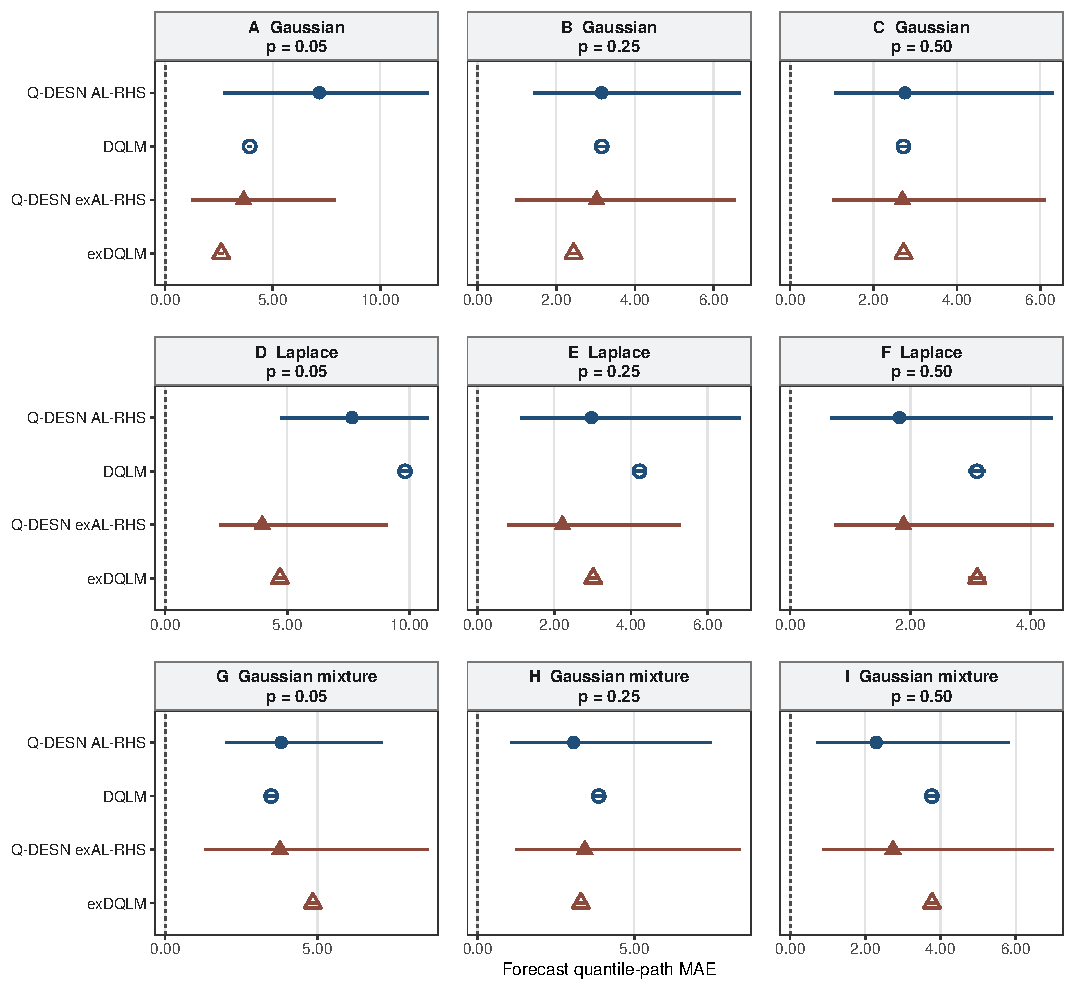
\includegraphics[width=0.98\textwidth]{figures/independent_simulation/qdesn_validation_500obs_v14_mcmc_forecast_mae_intervals.pdf}
\caption{MCMC posterior uncertainty for forecast MAE in the single-quantile
simulation. Horizontal segments show equal-tailed 95\% posterior intervals and
crosses show posterior means. Each panel has its own horizontal scale; lower is
better. The dashed line marks the exact DGP value of zero for quantile-path
error. Intervals condition on the simulated series, evaluation design, and
case-specific selected specification.}
\label{fig:simulation-500obs-mcmc-forecast-mae-intervals}
\end{figure}

\begin{figure}[!htbp]
\centering
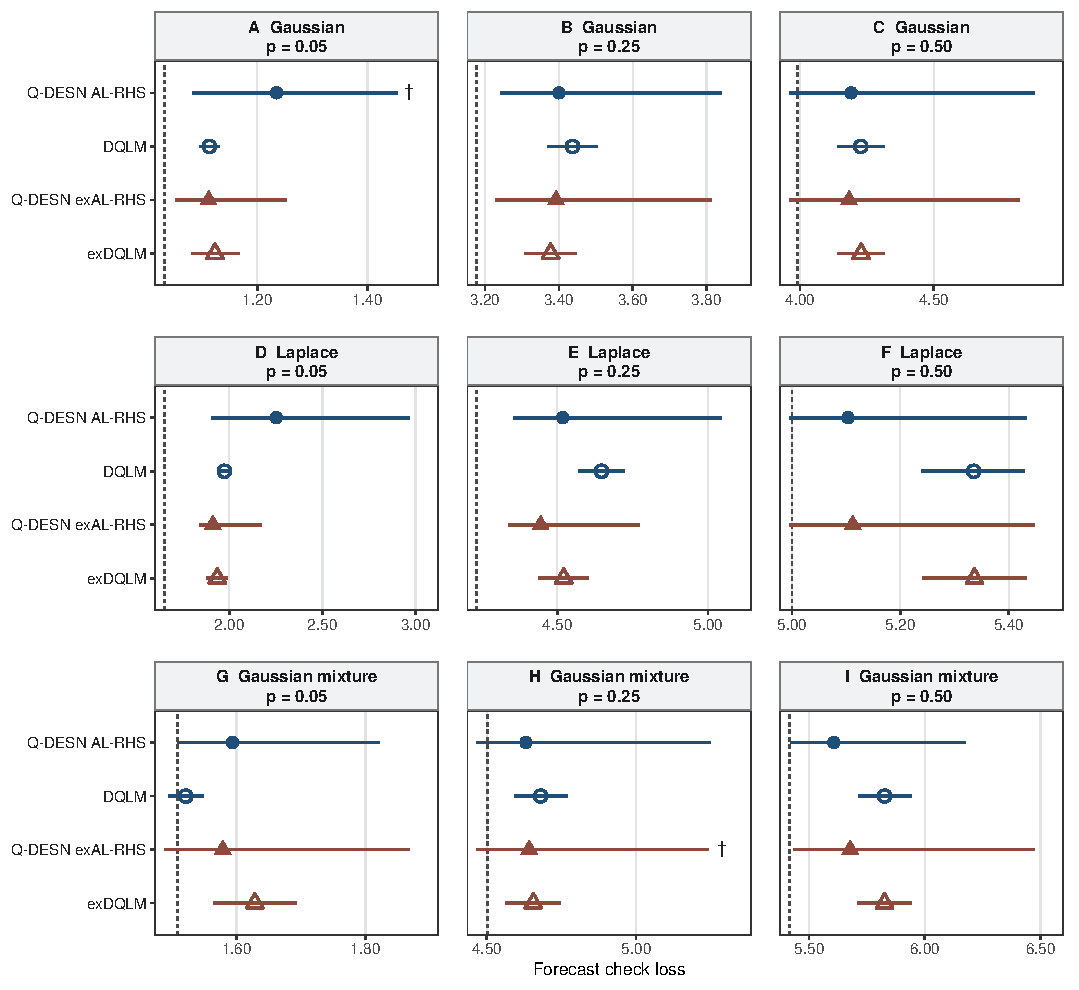
\includegraphics[width=0.98\textwidth]{figures/independent_simulation/qdesn_validation_500obs_v14_mcmc_forecast_check_loss_intervals.pdf}
\caption{MCMC posterior uncertainty for forecast check loss in the
single-quantile simulation. Horizontal segments show equal-tailed 95\%
posterior intervals and crosses show posterior means. Each panel has its own
horizontal scale; lower is better. The dashed line marks population expected
check loss at the true conditional quantile. Conditional finite-sample
intervals may cross this reference.}
\label{fig:simulation-500obs-mcmc-forecast-check-loss-intervals}
\end{figure}


\subsection{Joint Multi-Quantile Study with a Shared Feature Design}

The second simulation study compares joint and independent estimation of the
seven levels
\[
\tau\in\{0.05,0.10,0.25,0.50,0.75,0.90,0.95\}
\]
under the \(\AL\) and \(\exAL\) working likelihoods. Eight mechanisms span
Gaussian, Laplace, Gaussian-mixture, asymmetric-tail, persistent-heavy-tail,
Student-\(t\), regime-shift, and nonlinear dynamics. For each mechanism, one
DESN and RHS specification is selected using separate source realizations and
then shared by all four model classes. The 500-observation evaluation
realization is
not used for this selection. Thus differences among the 32 comparisons are
not confounded by model-specific feature maps or prior scales.

The evaluation fits use sequential initialization centered at the median.
A Gaussian ridge fit initializes Gaussian RHS--VB; the resulting compatible
estimates initialize the median \(\AL\) regression; and the remaining
independent \(\AL\) fits proceed toward the two tails. Each \(\exAL\) fit is
initialized from the \(\AL\) fit at the same level, the complete independent
grids initialize the corresponding joint fits, and each completed VB fit
initializes MCMC for the same model. These transfers determine starting values
only. The supplement gives the complete calculation and chain allocation.

Held-out evaluation is sequentially conditional: regression coefficients and
reservoir weights remain fixed, while newly observed response lags enter later
forecast origins. Each comparison contains the same 990 origin--horizon rows.
The primary criterion is \(S_{\mathrm{DGP}}\) in
Eq.~\eqref{eq:dgp-integrated-score-main}, computed for each retained MCMC draw
after monotone rearrangement. Independent quantile draws are combined by the
pre-specified chain-balanced product coupling described in the supplement.

Figure~\ref{fig:joint-qdesn-shared-backbone-forecast-score} shows the complete
posterior score comparison. Independent exQDESN has the smallest numerical
posterior mean in seven mechanisms; joint exQDESN is smallest for the Laplace
mechanism. The marginal intervals for the numerical winner and runner-up
overlap in every mechanism. Of the 16 paired joint-minus-independent
contrasts, five intervals favor independent estimation and eleven include
zero; none favors joint estimation. The evidence therefore does not support a
general forecast advantage from joint estimation under this shared design.

\begin{figure}[!htbp]
\centering
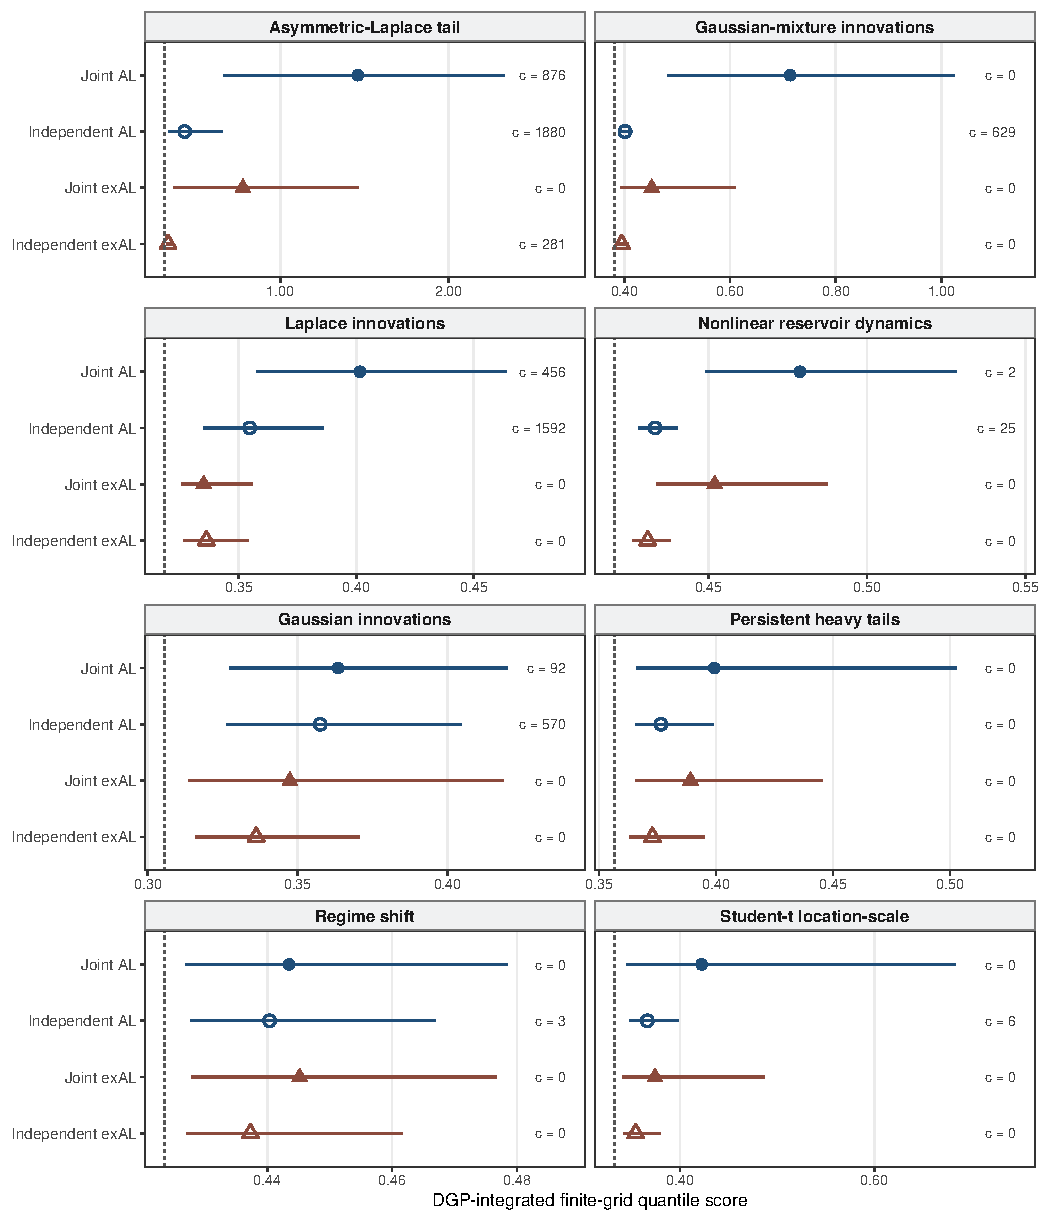
\includegraphics[width=0.94\textwidth]{figures/joint_qdesn_simulation/joint_qdesn_shared_backbone_forecast_dgp_score_intervals.pdf}
\caption{Posterior DGP-integrated finite-grid quantile scores under the shared-backbone design. Points are posterior means and horizontal bars are equal-tailed 95\% intervals; lower is better. Dashed lines mark the oracle finite-grid score. Filled symbols denote joint fits and open symbols independent fits; blue denotes \(\AL\) and red \(\exAL\). Labels \(c\) give raw crossings in the posterior-mean forecast grid; all counts after rearrangement are zero.}
\label{fig:joint-qdesn-shared-backbone-forecast-score}
\end{figure}


Before rearrangement, the posterior-mean forecast grids contain 1,426 crossings
for joint Q--DESN, 4,705 for independent Q--DESN, none for joint exQDESN, and
281 for independent exQDESN, summed over the eight mechanisms. Rearrangement
produces ordered grids in all 32 comparisons. Posterior-score diagnostics meet
the pre-specified criteria in 21 comparisons and warrant review in 11; all 16
\(\exAL\) scale--asymmetry assessments remain at review level. Exact scores,
fit recovery, crossing rates, and computational diagnostics are reported in
the supplement. A separate 50-replicate variational analysis is retained as a
sensitivity study.

\section{Application: GloFAS Retrospective Streamflow Quantile Forecasting}
\label{sec:data}

\noindent\textbf{Retrospective case study.}
We consider a medium-range streamflow forecast from the Global Flood Awareness
System (GloFAS), which is jointly developed by the European Commission and the
European Centre for Medium-Range Weather Forecasts and operated within the
Copernicus Emergency Management Service
\citep{AlfieriEtAl2013GloFAS,CEMS2026GloFASDocumentation}.
GloFAS provides ensemble river-discharge forecasts for flood early warning and
verification \citep{HarriganEtAl2023GloFASForecasts}. Q--DESN supplies a
statistical quantile correction relative to a United States Geological Survey
(USGS) gauge record at one forecast origin.

\subsection{Data and Forecast-Origin Design}

Let \(T\) be the forecast origin, \(y_t\) the transformed USGS record through
\(T\), \(g_t^{\mathrm{ret}}\) the retrospective GloFAS series, and
\(g_{T+h,m}^{\mathrm{ens}}\) issued ensemble member \(m\) at horizon \(h\).
The held-out \(y_{T+h}\) values are used only for evaluation. The analysis
uses origin \GlofasApplicationCurrentOriginDate{} and scores seven probability
levels over \GlofasApplicationCurrentScoredHorizons{} target dates. Its
covariate specification combines observed history and Global Ensemble Forecast System (GEFS) forecasts
with realized-future contributions to precipitation
and soil-moisture covariates. This blended information set makes the analysis
retrospective; it does not represent a real-time forecast based only on
information available at \(T\).

\subsection{Application Model}

\noindent\textbf{Persistence-anchored discrepancy.}
Two fixed Q--DESN feature maps represent the reference history and the
retrospective discrepancy \(g_t^{\mathrm{ret}}-y_t\). For \(t>T\), the
persistence-plus-adjustment specification anchors the future discrepancy
feature at its last historical value; subsequent discrepancy features describe
adjustments around that persistence-anchored discrepancy baseline. For
probability level \(p_0\),
\[
q^{\mathrm{ref}}_{p_0,t}=\vect x_t^{\mathrm{ref}\top}\vect\beta_{p_0},
\qquad
d^{\mathrm{glo}}_{p_0,t}=\vect x_t^{\mathrm{disc}\top}\vect\alpha_{p_0},
\qquad
q^{\mathrm{glo}}_{p_0,t}=q^{\mathrm{ref}}_{p_0,t}+d^{\mathrm{glo}}_{p_0,t}.
\]
The reference-process quantile \(q^{\mathrm{ref}}_{p_0,t}\) is the scored
quantity, and \(d^{\mathrm{glo}}_{p_0,t}\) is the quantile-specific GloFAS
discrepancy. The reported analysis fits the seven levels \(0.05\), \(0.15\),
\(0.35\), \(0.50\), \(0.65\), \(0.80\), and \(0.95\) independently with AL
working likelihoods, separate RHS hierarchies for the two coefficient blocks,
and VB. Issued ensemble members are treated as conditionally independent and
exchangeable given the forecast-system quantile path, a working-likelihood
approximation because the members arise from perturbed initial conditions and
model perturbations \citep{ECMWF2026ENSGeneration}. Variational posterior-mean
quantile estimates are monotonically rearranged on the fitted grid. The
supplement gives the source-specific likelihood, the fixed reservoir
specifications, and the more general exAL and latent-future-path formulations.

\subsection{Retrospective Application Results}

The reported fit was evaluated over
\GlofasApplicationCurrentObservedHistoryDates{} observed dates through the
forecast origin. After monotone rearrangement, its observational-window
\(\aCRPS\) was \(\GlofasApplicationCurrentObservedHistoryAcrps{}\), and
empirical 90\% interval coverage was
\(\GlofasApplicationCurrentObservedHistoryCoverage{}\). These fitting-period
scores were used for model selection, with the forecast period reserved for
evaluation. The fitted \(p_0=0.95\) quantile occasionally takes extreme values
in the observational period, so upper-tail forecasts are interpreted
cautiously.

\noindent\textbf{Forecast-period scores.}
Table~\ref{tab:glofas-application-score} shows lower mean check loss, interval
score, and \(\aCRPS\) for Q--DESN than for raw GloFAS at this origin. Empirical
coverage of the nominal 90\% interval is
\(\GlofasApplicationCurrentQdesnMeanCoverage{}\) for Q--DESN and
\(\GlofasApplicationCurrentRawMeanCoverage{}\) for raw GloFAS. The improvement
from zero coverage does not resolve the substantial Q--DESN undercoverage.
Multi-origin evaluation using only covariates available at each origin is
needed to assess real-time performance and calibration.

\begin{table}[!htbp]
\centering
\caption{Forecast scoring for the GloFAS retrospective analysis.
Scores are computed on the transformed streamflow scale for the
forecast origin \GlofasApplicationCurrentOriginDate{}. Lower check loss,
interval score, and \(\aCRPS\) are better; \(\aCRPS\) is computed from
Eq.~\eqref{eq:acrps-main} at seven common evaluation levels. Mean
coverage reports empirical coverage for the nominal 90\% interval and
is interpreted descriptively. The final column gives the relative reduction in
mean check loss.}
\label{tab:glofas-application-score}
\input{\GlofasApplicationCurrentScoreTable}
\end{table}

\begin{figure}[H]
\centering
\includegraphics[width=0.94\textwidth]{\GlofasApplicationCurrentForecastWindowFigure}
\caption{Q--DESN quantile intervals for the GloFAS retrospective analysis over
the final 60 observed dates and the following 28-day forecast period. The
nested blue bands are the 90\%, 65\%, and 30\% quantile intervals, and the blue
path is the median. The vertical dashed line marks the forecast origin. Black
and red paths denote observed and held-out USGS streamflow, respectively;
orange denotes retrospective GloFAS, and thin gray paths show all 51 issued
GloFAS ensemble members, with their median dashed. Forecast scores use the
held-out measurements in Table~\ref{tab:glofas-application-score}.}
\label{fig:glofas-application-forecast-period}
\end{figure}

\section{Application: PriceFM Retrospective Electricity-Price Comparison}
\label{sec:pricefm-application}

The second application compares retrospective Q--DESN day-ahead
electricity-price forecasts with version~4 of PriceFM
\citep{YuEtAl2026PriceFM}. The release covers European bidding regions at
15-minute resolution from 1~January~2022 through 1~January~2026 and includes
price, load, solar, and wind forecasts. Average quantile loss (AQL) is evaluated
on the PriceFM probability grid at matched held-out timestamps for 114
region--fold comparisons.

\subsection{Comparison Design}

The comparison contains \PricefmFullRegionFolds{} region--fold
evaluations, spanning \PricefmFullRegions{} European bidding regions and
\PricefmFullFolds{} rolling folds. Each evaluation is scored on the
fold-aligned held-out timestamps and probability levels
\PricefmFullPaperQuantiles. Throughout this section, \(\Delta\) AQL denotes
Q--DESN AQL minus PriceFM AQL. Negative values indicate lower Q--DESN AQL;
positive values indicate lower PriceFM AQL.

\noindent\textbf{Retrospective covariates.}
We compare Q--DESN forecasts with the released PriceFM forecasts at matched
region--fold timestamps. Across the comparison, \PricefmFullTargetOnlyRows{}
evaluations use own-region predictors and \PricefmFullGraphRows{} evaluations
also include neighboring-region summaries. Both predictor sets use retrospectively
observed own-region load, solar, and wind lead covariates in the comparison;
evaluations with neighborhood summaries add retrospectively observed neighboring-region lead
summaries. The score comparison is therefore retrospective. A PriceFM study of the
joint quantile-vector RHS prior would require the same fold-aligned design with
that joint regression fitted directly.

\subsection{Results by Region, Fold, and Forecast Lead}

Across the aligned benchmark, Q--DESN has lower AQL in
\PricefmFullQdesnWins{} of \PricefmFullRegionFolds{} region--fold evaluations
(\PricefmFullQdesnWinRate{}). Relative to its own AQL, PriceFM has lower AQL by
at most 5\% in \PricefmFullQdesnClose{} comparisons and by more than 5\% in
\PricefmFullPricefmWins{} comparisons. The mean Q--DESN AQL is
\PricefmFullMeanQdesnAql{}, compared with mean PriceFM AQL
\PricefmFullMeanPricefmAql{}, giving mean \(\Delta\) AQL
\PricefmFullMeanDeltaAql{} and median \(\Delta\) AQL
\PricefmFullMedianDeltaAql{}. The differences vary across region--fold
comparisons. Within \PricefmSelectionComparedRows{} region--fold
comparisons, AL and exAL specifications were chosen using validation AQL and
then evaluated on held-out observations. The validation-selected
specifications averaged test AQL \PricefmSelectionCandidateMeanAql{}, compared
with \PricefmSelectionReferenceMeanAql{} for the reference Q--DESN
specifications. The reported aggregate uses the selected specification in
\PricefmSelectionUpdatedRows{} cases
in which its held-out AQL was lower than both the reference Q--DESN and matched
PriceFM values. Because held-out performance determined these 12
substitutions, the resulting aggregate is descriptive; complete case-level
results are reported in the supplement.

Across the 114 region--fold comparisons, the unweighted mean AQCR is
\PricefmAlignedQdesnAqcr{} for Q--DESN and
\PricefmAlignedPricefmAqcr{} for PriceFM. Mean MAE is
\PricefmAlignedQdesnMae{} for Q--DESN and \PricefmAlignedPricefmMae{} for
PriceFM; mean RMSE is \PricefmAlignedQdesnRmse{} and
\PricefmAlignedPricefmRmse{}, respectively. Relative to PriceFM, Q--DESN has
\PricefmAlignedAqlReduction{}, \PricefmAlignedMaeReduction{}, and
\PricefmAlignedRmseReduction{} lower mean AQL, MAE, and RMSE, respectively.
Table~\ref{tab:pricefm-matched-aql-comparison} summarizes the AQL results
overall, by fold, and by forecast-lead block.

\begin{table}[!htbp]
\centering
\caption{Matched retrospective comparison of Q--DESN and PriceFM. Panel~A
reports unweighted summaries across region--fold comparisons, overall and by
fold. The two PriceFM columns distinguish
\(0<\Delta\mathrm{AQL}/\mathrm{AQL}_{\mathrm{PriceFM}}\leq 0.05\) from
relative differences greater than 0.05.
Panel~B reports paired AQL differences for the 72 region--fold comparisons with
forecast-lead-specific results. Its means and medians are unweighted summaries
of the 72 paired differences in each forecast-lead block. At 15-minute
resolution, the four successive 24-step blocks each span six hours. Here
\(\Delta\) AQL is Q--DESN minus PriceFM, so negative values favor Q--DESN.
AQL is in EUR/MWh, and all scores use matched held-out timestamps and the same
seven probability levels.}
\label{tab:pricefm-matched-aql-comparison}
\noindent\textit{Panel A: Overall and fold-specific results}\par\smallskip
\begin{tabular}{lrrrrrrrr}
\toprule
Scope & Rows & Q--DESN wins & Near ties & PriceFM wins & Q--DESN AQL & PriceFM AQL & Mean $\Delta$ & Median $\Delta$ \\
\midrule
Overall & 114 & 66 & 12 & 36 & 6.826 & 7.039 & -0.213 & -0.083 \\
Fold 1 & 38 & 22 & 6 & 10 & 7.047 & 7.297 & -0.250 & -0.073 \\
Fold 2 & 38 & 30 & 2 & 6 & 6.429 & 6.826 & -0.397 & -0.295 \\
Fold 3 & 38 & 14 & 4 & 20 & 7.001 & 6.993 & 0.008 & 0.281 \\
\bottomrule
\end{tabular}
\par
\medskip
\noindent\textit{Panel B: Results by forecast-lead block}\par\smallskip
\begingroup
\TableStyle
\scriptsize
\setlength{\tabcolsep}{3pt}
\begin{tabular}{@{}lrrrr@{}}
\toprule
Horizon block & $n$ & \shortstack{Q--DESN\\lower} & \shortstack{Mean\\$\Delta$} & \shortstack{Median\\$\Delta$} \\
\midrule
1-24 & 72 & 22 & 0.415 & 0.351 \\
25-48 & 72 & 45 & -0.684 & -0.382 \\
49-72 & 72 & 34 & -0.198 & 0.032 \\
73-96 & 72 & 42 & -0.155 & -0.114 \\
\bottomrule
\end{tabular}
\endgroup
\par
\end{table}

Mean Q--DESN AQL is lower in folds 1 and 2 and nearly equal in fold 3.
Evaluations with neighborhood summaries have a more negative mean
\(\Delta\) AQL than own-region-only evaluations. Forecast-lead-specific results
are available for 72 of the 114 comparisons: PriceFM is favored in the first
six-hour block, whereas the later blocks favor Q--DESN on average but remain
heterogeneous across regions and folds. The differing predictor sets,
case-specific specifications, and incomplete lead-specific panel make these
comparisons descriptive.

In this retrospective comparison, Q--DESN has lower aggregate AQL, MAE, and
RMSE than the matched PriceFM forecasts, with substantial variation across
folds, regions, and forecast horizons. Paired uncertainty analyses and direct
evaluation of the joint quantile model remain topics for future study.

% ============================================================
\section{Discussion}
\label{sec:discussion}

Q--DESN treats the fixed DESN reservoir as a nonlinear feature map and places
Bayesian quantile inference on the regression coefficients. Posterior
simulation and variational inference concern the regression, likelihood, and
shrinkage parameters conditional on the fixed reservoir features. The empirical
results evaluate this conditional Bayesian quantile-regression analysis under
specified reservoir constructions.

The AL and exAL families are used as working likelihoods for conditional
quantiles. They provide posterior distributions and conditionally tractable
augmented updates. The
simulation and application sections report fit recovery, forecast scoring,
empirical predictive coverage, monotonicity, and convergence diagnostics to
assess the model-based summaries under possible misspecification. Sandwich
corrections and generalized-Bayes calibration for composite quantile
likelihoods remain important topics for further study.

The multi-quantile construction makes the same distinction. Independent
single-level Q--DESN fits followed by isotonic regression or rearrangement
produce monotone quantile curves from level-wise regressions. The joint
quantile-vector extension shares information across quantile levels through RHS
shrinkage on adjacent coefficient differences. This shrinkage can reduce
crossings but does not enforce monotonicity. Ordered parameterizations or
monotone rearrangement can be used when monotonicity is required.

The single-quantile dynamic simulations assess recovery and held-out
forecasting under known data-generating mechanisms. The joint multi-quantile
study assesses quantile-path recovery and crossings under known conditional
quantile paths. The GloFAS application studies one
retrospective streamflow forecast origin with independent Q--DESN AL--VB fits,
blended future weather covariates, monotone reporting, and undercoverage of the
nominal 90\% interval. The PriceFM comparison uses matched PriceFM forecasts with
retrospectively observed lead covariates. Broader
rankings of Q--DESN against dynamic quantile or foundation-model alternatives
require evaluations across additional data sets, forecast origins, and
reservoir specifications.

Several extensions are natural. On the statistical side, future work should
study calibrated composite-likelihood scaling, hard or probabilistic
non-crossing constraints, richer covariance structures for quantile
differences, and sensitivity to reservoir scaling on bounded feature domains.
On the computational side, the joint model calls for sparse precision solvers,
targeted covariance extraction for VB, and diagnostics comparing VB with
MCMC on small joint problems. On the application side, multi-origin operational
GloFAS studies with covariates known at the forecast origin, paired PriceFM
uncertainty analyses, and explicitly joint PriceFM analyses are needed before the joint
quantile-vector prior can be interpreted in an application-level benchmark.

Q--DESN combines fixed nonlinear recurrent features with Bayesian regression
for dynamic conditional quantiles. The results demonstrate conditional-quantile
estimation under the specified simulation designs and retrospective
applications and identify the settings requiring broader validation.

% ============================================================
\bibliographystyle{apalike}
\bibliography{refs}

\end{document}
